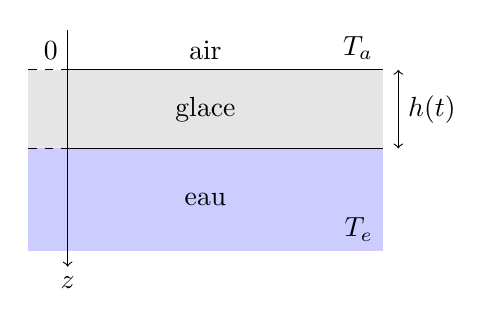
\begin{tikzpicture}
	% Lac gelé
	\fill[gray!20] (-0.5, 0) rectangle (4, -1) node[black, midway] {glace};
	\fill[blue!20] (-0.5, -1) rectangle (4, -2.3) node[black, midway] {eau} node[above left, black] {$T_e$};
	\node[above] at (1.75, 0) {air};
	\draw (0, 0) node[above left] {$0$} -- (4, 0) node[above left] {$T_a$};
	\draw (0, -1) -- (4, -1) ;
	\draw[dashed] (-0.5, 0) -- (0,0) (-0.5, -1) -- (0, -1);
	\draw[->] (0, 0.5) -- (0, -2.5) node[below] {$z$};
	\draw[<->] (4.2, 0) -- (4.2, -1) node[midway, right] {$h(t)$};
\end{tikzpicture}